\chapter{New Approaches for Generating Visualizations and Applications}
\label{ch:ch5}

\begin{itemize}
\item Survey on visualizations for RDF
\item Contrib 1: Wizard for visualizations
\item Contrib 2: Vocabularies for describing visualizations (added)
\item Contrib 4: Revealing the ``important'' properties of Entities for visualizations (added)
\item Contrib 5: Focus on Event--Confomaton
\item Contrib 6: Focus on statistics -Concrete applications: PerfectSchool, French Amenities.
\item Contrib 7: Apps4Europe: Improving the discovery of application contests in Open Data Events

\end{itemize}

\section{Wizard for Visualizations}

%\ghis{find a good justifying example} \\

With the growing adoption of the Linked Data principles, there is a real need to support data consumers in quickly getting visualizations that enable to explore a dataset. In order to involve more general Web users into the Semantic Web and Linked Data world, there is a need to build tools that reuse existing visualization libraries showing the key information about RDF datasets. Many datasets are published using SPARQL Endpoints and are not ``visually'' accessible. Thus, understanding the underlying graphs and consuming them require lay users to have some knowledge in writing queries. 

The object of visualization is to develop insights from collected data. Moreover, according to Information Theory, vision is the sense that has the largest bandwidth (100 Mbits/s), which makes it the best suited channel to convey information to the brain \cite{Ware:2014}. Based on the Visual Information Seeking Mantra: \textit{``overview first, zoom and filter, then details on demand''} \cite{Shneiderman99}, we advocate for more visual interactive representations of RDF graphs using SPARQL Endpoints.   At the same time,  we use the term ``Linked Data Visualization'', to refer to a \textit{combination of charts, graphics, and other visual elements built on top of 4-5 stars datasets accessible via a SPARQL endpoint}. 
Despite the presence of more and more datasets published as Linked Data, there is still a need to help end users to discover what (unknown) datasets describe by hiding the complexity of SPARQL queries from such users. Moreover, the task of identifying the key categories of datasets can help in selecting and matching the most suitable visualization types.

In this Section, we propose a first step towards making available a semi-automatic way for the production of possible visualization of linked data sets of high-level categories grouping objects that are worth viewing and we associate them with some very well known vocabularies. Then, we describe the implementation of a Linked Data Visualization Wizard and its main components. This wizard can be used to easily visualize slices of datasets based on generic types detected.

The remainder  of this paper is structured as follows. We first provide some related work that further motivates this study (Section~\ref{sec:related}). In Section~\ref{sec:vizTypes}, we propose some important categories that are worth visualizing and we present a set of mapping views associated with vocabularies (Section~\ref{sec:mapping}). In Section~\ref{sec:ldvizwiz}, we describe the implementation of a wizard that can work on top of any RDF dataset. We detail the results of an experiment where high level categories and associated visualizations have been performed on numerous SPARQL endpoints (Section~\ref{sec:evaluation}). 

\subsection{Dataset Analysis}
\label{sec:vizTypes}
When developing an application, there are some ``important'' classes/categories, objects or datatypes that can be detected first to help to guide in the progress of creating a set of visualizations tied with those categories. We distinguish seven categories while acknowledging that this is not necessary an exhaustive list:
\begin{itemize}
 \item{\S~[\textbf{Geographic information}]}: This category is for data modeled using \texttt{geo:SpatialThing}, \texttt{dbpedia-owl:Place}, \texttt{schema:Place} or \texttt{gml:\_Feature} classes.
 \item{\S~[\textbf{Temporal information}]}: This category also includes dataset containing date, time (e.g: \texttt{xsd:dateTime}) and period or interval of time, using the OWL Time ontology.
 \item{\S~[\textbf{Event information}]}: This category is for any action of activity occurring at some place at some time.
 \item{\S~[\textbf{Agent/Person information}]}: This category is heavily influenced by the use of \texttt{foaf:Person} or \texttt{foaf:Agent}.
 \item{\S~[\textbf{Organization information}]}: This category is related to organizations or companies data, with the use of the \texttt{org} vocabulary\footnote{\url{http://www.w3.org/TR/vocab-org/}} or the \texttt{foaf:Organization} class.
 \item{\S~[\textbf{Statistics information}]}: This category refers to statistical data generally modeled using the \texttt{data cube} vocabulary\footnote{\url{http://www.w3.org/TR/vocab-data-cube/}} or the SDMX model\footnote{\url{http://sdmx.org/}}.
 \item{\S~[\textbf{Knowledge Classification}]}: This category refers to dataset describing schemas, classifications or taxonomies using the \texttt{SKOS} vocabulary.
\end{itemize}



\section{Mapping Datatype, Views and Vocabularies}
\label{sec:mapping}
%\todo{add ref. to "Interactive Data Visualization" by Ward et al.}

The On-line Library of Information Visualization Environments (OLIVE)\footnote{\url{http://lte-projects.umd.edu/Olive/}} is a web site describing eight categories of information visualization environments differentiated by data type and collected by students, following a visualization course given at Maryland College Park, mostly inspired from the work of Ben Shneiderman \cite{Shneiderman99}. Based on the classification provided by OLIVE, we propose a set of mappings between those categories (excluding the workspace dimension), views that can be applied to this category and a suitable list of vocabularies from the Linked Open Vocabularies catalogue \cite{lov11}\footnote{\url{lov.okfn.org/dataset/lov/}} that correspond to those categories. Those vocabularies are easy to be found as there is a manual classification of vocabularies by the curators of the catalogue based on the content and scope of the terms and properties. According to the seven categories defined in Section ~\ref{sec:vizTypes}, we have identified some of their corresponding one to one mapping with the set of vocabularies:
 \begin{itemize}
 \item \textbf{Geography} space, consisting of 21 vocabularies for features: \texttt{geo}, \texttt{gn}, \texttt{gf}, \texttt{om}, \texttt{geop}, \texttt{md}, \texttt{lgdo}, \texttt{loc}, \texttt{igeo}, \texttt{osadm}, \texttt{geod}, \texttt{ostop}, \texttt{place}, \texttt{geos}, \texttt{locn}, \texttt{coun}, \texttt{postcode}, \texttt{osr}, \texttt{geof}, \texttt{g50k} and \texttt{ad}.
 \item \textbf{Geometry} space, for vocabularies dealing with the geometries, mostly combined with the features, such as: 
 \item \textbf{Time} space, consisting of 14 vocabularies, such as \texttt{cal}, \texttt{date}, \texttt{gts}, \texttt{interval}, \texttt{ncal}, \texttt{oh}, \texttt{te}, \texttt{thors}, \texttt{ti}, \texttt{time}, \texttt{tl}, \texttt{tm}, \texttt{tvc} and \texttt{tzont}. 
 \item \textbf{Event} space, containing vocabularies such  as \texttt{event}, \texttt{lode}, \texttt{music}, \texttt{sem}, \texttt{situ}, \texttt{sport}, \texttt{stories}, \texttt{theatre}, \texttt{tis} and \texttt{tisc}.
 \item \textbf{Government} space, with 9 vocabularies (\texttt{cgov}, \texttt{ctorg}, \texttt{elec}, \texttt{few}, \texttt{gc}, \texttt{gd}, \texttt{oan}, \texttt{odd}, \texttt{parl}) and the \texttt{org} vocabulary belonging to the W3C recommendation vocabularies at \url{ http://lov.okfn.org/dataset/lov/lov#W3C}.
 \end{itemize} 
 Metadata vocabularies, such as \texttt{rdfs}, \texttt{dcterms} or \texttt{dce} can be used in association with any of the visual element to give basic description of the resource of a giving dimension. For example, a popup information can be fired on a map view to display the relevant information of a geodata resource such as the label, the abstract or description. 
Another application can be to detect which visualization is best suited for geodata. Geodata belongs to a  two-Dimension visual representation. Geodata is usually displayed using geographical-based visualizations (map, geo charts, etc.) and it is often modeled by vocabularies in the space named \texttt{Geometry} and \texttt{Geography}\footnote{All the prefixes used for the vocabularies are the same used in LOV catalogue.}   vocabularies in RDF datasets. Hence those vocabularies can be combined to detect the presence or not of geographic information in a dataset, and thus yield to recommend a map view. Table~\ref{tab:taxonomy} gives an overview of those mappings. For the tabular representation, it is the ``default'' visual representation of RDF data and can be used by any vocabulary without restriction. 


\begin{table}[!htbp]
\centering{
\begin{tabular}{lllc}
 \specialrule{1pt}{1pt}{1pt}
 \textbf{Dimension}	 	& \textbf{Vocabulary Space}  & \textbf{Visual element}		 \\ \specialrule{1pt}{1pt}{1pt}
 Temporal 	     &  \textsf{Time space} &     TimeLine		      	 		 \\
 one-Dimension  & \textsf{any}	   & Tabular, text							 \\
 two-Dimension   & \textsf{Geography space}     & Map view 						\\
 			& \textsf{Geometry space}    & Maps view                            \\
 three-Dimension  	& \textsf{Event space}  	& Map + TimeLine	 			\\
 Multi-Dimension  & \textsf{qb}, \textsf{sdmx-model}, \textsf{scovo}      & Charts, graphs   			 		\\
 Tree	      &   \textsf{skos, Government space}            & Treemap, Org view   				\\
 Network	  & \textsf{any vocab.}   & Graph, network map  			 			
 \\
 \specialrule{1pt}{1pt}{1pt}
\end{tabular}
\caption{A taxonomy of information visualization consuming Linked Datasets with associated views and suitable vocabulary space.}
\label{tab:taxonomy}
}
\end{table}


\section{LDVizWiz: a Linked Data Visualization Wizard}
\label{sec:ldvizwiz}

%\todo{present in detail the queries for detecting ALL the categories} \\

We propose a workflow composed of four principal steps for a Linked Data Visualization Wizard, as depicted in Figure~\ref{fig:workflow}. Our requirement is to provide a tool that hide the complexity of SPARQL to lay users and at the same time, can be embedded in existing Linked Data infrastructure and workflow. First, we proposed to detect the presence of data belonging to one of the seven categories (Table~\ref{tab:taxonomy}) using generic SPARQL queries. More precisely, we perform \texttt{ASK} queries to test whether or not a particular query pattern has a solution. Second, we look at entities in a dataset that have \texttt{owl:sameAs} links with external objects and we retrieve the properties associated to those objects. We argue that the objects that are interlinked with other datasets are of primary importance in a visualization. We show the results of this mining process to the user (the categories that have been detected, the properties going with the categories and the external domain). Based on this information, the user can make a personalized ``mashup'' by aggregating the suitable visualization widgets. Some default visualizations are available according to the top categories detected. The last step is to publish the visualization and a metadata report in RDF/XML TURTLE or N3.

\begin{figure*}[!htbp]
\begin{center}
\subfigure[The workflow of the different modules interacting in the Linked Data visualization wizard.]{
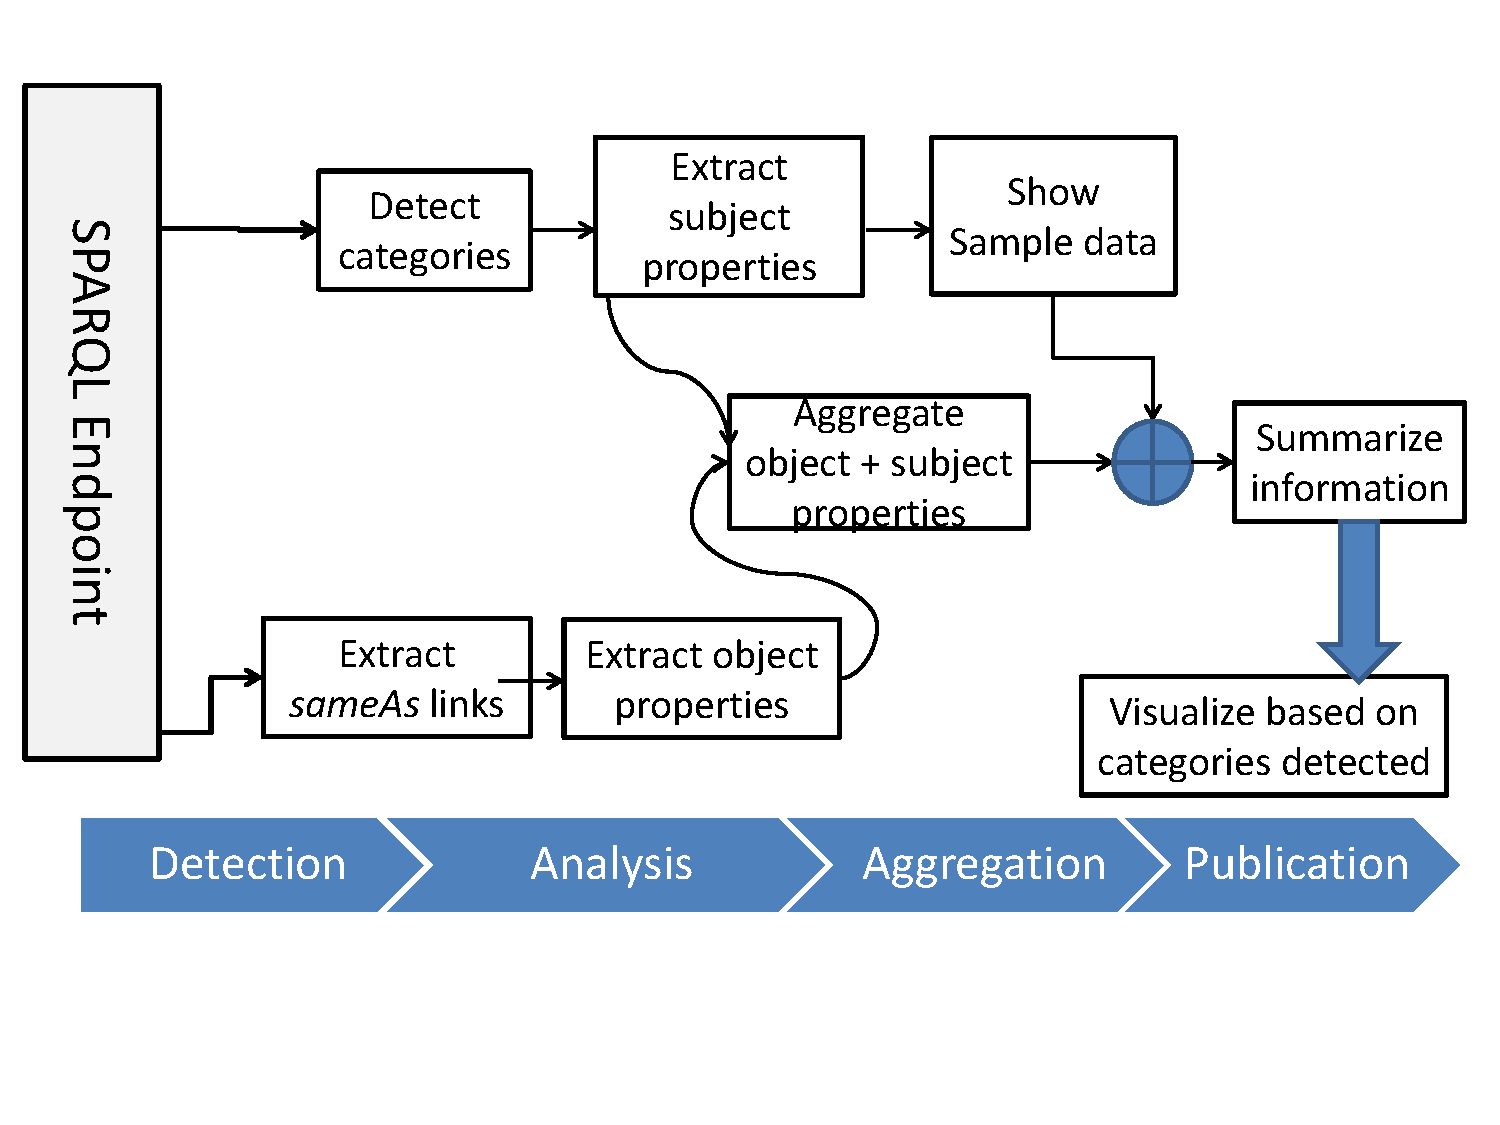
\includegraphics[width=0.5\textwidth]{img/workflow-visu.pdf}
}
\subfigure[High level functionalities of the Linked Data visualization wizard ]{
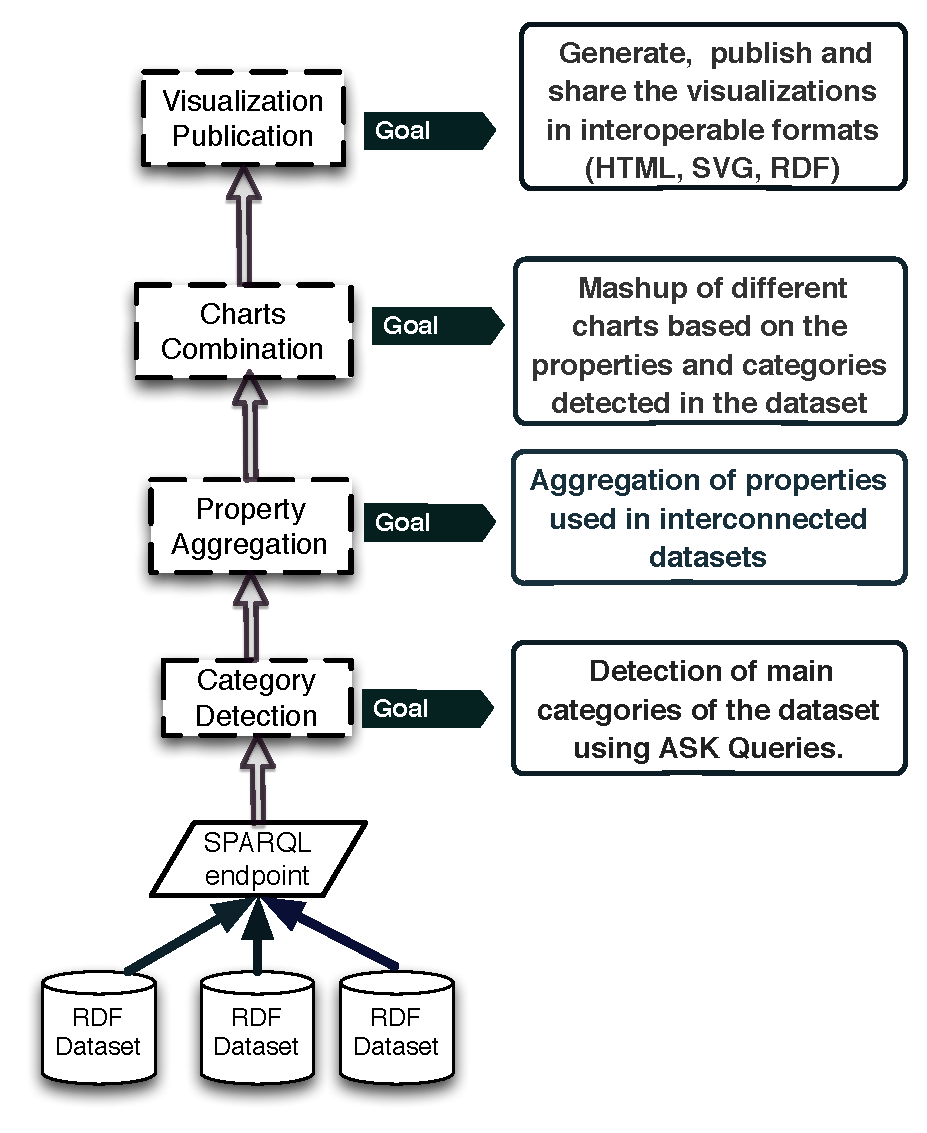
\includegraphics[width=0.4 \textwidth]{img/architecture-ldwizard.pdf}
}


\caption{Big picture and architecture of the Linked Data visualization wizard.}
\label{fig:workflow}
\end{center}
\end{figure*}

Let consider a graph $<G,c>$ to be $G=\{(s,p,o)| p \in URI, s \in URI, o \in (URI \cup LIT)\} $ where $URI$ is the set of URIs, $LIT$ is the set of literals, and $c$ the context. We define $L=\{V_{1}, V_{2}, ...,V_{n} | V_{i}=P_{i} \cup T_{i}\} $ the list of vocabularies in LOV, with $P_{i}$ and $T_{i}$ respectively the properties and terms of a vocabulary $V_{i}$. Let also $D=\{D_{1}, D_{2}, ..,D_{m} \} $ be the domains of vocabularies. We assume $ \forall V \in L, \exists D_{k} \in \Phi(L,D) $. We define a generic function $\Sigma:(G,c)\mapsto B $ to detect categories in a dataset as follows: $\Sigma((G,c))=\{B| ( \exists(s,p,o) \in G: p \in V) \cup (\exists(s, rdf:type,o) \in G: o \in V)\} $ where $B =\{True, False\} $.


In the following sections, we describe each of the steps involved in the Linked Data Visualization Wizard in more details. 

\subsection{Category Detection}
The goal of the category detection task is to use SPARQL queries to detect the presence of some high level categories in the dataset. We perform \texttt{ASK} queries as implementation of the $\Sigma $ function using standard vocabularies as defined in the Table~\ref{tab:taxonomy}. We start with six categories, namely: geographic information, person, organization, event, time and knowledge organization systems. We select popular vocabularies based on two existing catalogues: LOV~\cite{pyv2012} and prefix.cc\footnote{\url{http://prefix.cc}}.

%asking geodata
\lstset{basicstyle=\scriptsize, backgroundcolor=\color{white}, frame=single, caption= {Generic query to detect geo data from a SPARQL endpoint}, label=geodata, captionpos=b}
\begin{lstlisting}
ASK WHERE {
 {
  ?x a ?o.
  filter (?o= dbpedia-owl:Place ||
    ?o=gml:_Feature || 
    ?o=geo:SpatialFeature || ?o=gn:Feature ||
    ?o=admingeo:CivilAdministrativeArea ||
    ?o=spatial:Feature ||
    ?o=vcard:Location)
 }
 UNION {
  ?x ?p ?o. filter(?p=geo:lat || ?p=geo:long ||
  ?p=georss:point || ?p=geo:geometry || 
  geom:geometry)
 }
}
\end{lstlisting}

 Listing~\ref{geodata} shows seven classes of different vocabularies are used, respectively for the namespaces \texttt{dbpedia-owl, geo, gn, admingeo, spatial} and \texttt{vcard}, with relevant classes to check the presence of geographic data.

\lstset{basicstyle=\scriptsize, backgroundcolor=\color{white}, frame=single, caption= {Generic query to detect time data from a SPARQL endpoint, using \texttt{time, dbpedia-owl, intervals} vocabularies.}, label=timedata, captionpos=b}
\begin{lstlisting} 
	ASK WHERE {{?x a ?o. filter(?o=time:TemporalEntity || 
	?o=time:Instant || 
		?o=time:Interval || ?o=dbpedia-owl:TimePeriod || 
		?o=time:DateTimeInterval || ?o=intervals:CalendarInterval)
	} 
	UNION{ ?x ?p ?o. filter(?p=time:duration || 
	?p=time:hasBeginning || 
	?p=time:inDateTime || ?p=time:hasDateTimeDescription 
	|| ?p=time:hasEnd)}

\end{lstlisting}

Listing \ref{timedata} detects the presence of time information, while Listing \ref{persondata}, \ref{orgdata} and \ref{eventdata} detect persons, organizations and events respectively.

\lstset{basicstyle=\scriptsize, backgroundcolor=\color{white}, frame=single, caption= {Generic query to detect person categories from a SPARQL endpoint, using \texttt{foaf, dbpedia-owl, vcard} vocabularies.}, label=persondata, captionpos=b}
\begin{lstlisting}
	ASK WHERE {?x a ?o. filter(?o = foaf:Person ||
	 ?o=dbpedia-owl:Person ||
		?o=vcard:Individual) }
	
\end{lstlisting}

\lstset{basicstyle=\scriptsize, backgroundcolor=\color{white}, frame=single, caption= {Generic query to detect ORG data from a SPARQL endpoint.}, label=orgdata, captionpos=b}
\begin{lstlisting}
PREFIX org:<http://www.w3.org/ns/org#>
	PREFIX foaf: <http://xmlns.com/foaf/0.1/> 
	PREFIX dbpedia-owl: <http://dbpedia.org/ontology/> 
	ASK WHERE {?x a ?o . filter (?o=org:Organization || 
	?o=org:OrganizationalUnit || 
	?o=foaf:Organization || 
	?o=dbpedia-owl:Organisation)}
	
\end{lstlisting}	

\lstset{basicstyle=\scriptsize, backgroundcolor=\color{white}, frame=single, caption= {Generic query to detect event data from a SPARQL endpoint, using \texttt{lode, event, dbpedia-owl} vocabularies.}, label=eventdata, captionpos=b}
\begin{lstlisting}
    ASK WHERE{?x a ?o. filter (?o= lode:Event || ?o=event:Event || 
    ?o=dbpedia-owl:Event)}	
    
  \end{lstlisting}
  
  
For detecting data organized as taxonomy, \texttt{skos} vocabulary is used along with the most used classes and properties as showed in Listing \ref{skosdata}.

\lstset{basicstyle=\scriptsize, backgroundcolor=\color{white},
frame=single, caption= {Generic query to detect SKOS data from a SPARQL endpoint, using \texttt{skos} vocabulary.}, label=skosdata, captionpos=b}
\begin{lstlisting}
    ASK WHERE {{?x a ?o. filter(?o=skos:Concept ||
     ?o=skos:ConceptScheme || ?o=skos:Collection )}
    	 UNION{ ?x ?p ?o. filter(?p=skos:featureCode || 
    	?p=skos:altLabel || ?p=skos:prefLabel  || ?p=skos:relatedMatch)}}		
\end{lstlisting}


\subsection{Property Aggregation}
We take the benefits of the \texttt{owl:sameAs} links between entities to have access to the properties of the entities in the external namespaces different from the origin dataset. This module also aggregates the properties found in the dataset with the ones found in the interlinked sets. This is based on the assumption that during the linkage process, external datasets not only help in not breaking the \textit{follow-your-nose} principle, but also add more information to be viewed in visualization applications. As shown in the code below, at this stage, we have collected and aggregated external properties gathered from the enrichment process of the workflow.

\begin{verbatim}
1-LET Namespace(?s) = S and LET Namespace(?t) =T
2-SELECT  owl:sameAs links
	LET SEMTERM = list of ?s owl:sameAs ?t
	WITH T != S
3-IN T, SELECT distinct properties used in dataset
4-AGGREGATE (3) with properties FROM S.
\end{verbatim}

\subsection{Visualization Generator}
This module aims at recommending the appropriate visualizations based on the categories detected by the wizard. It might also help the user to make a report summarizing the result of the mining process, and then use different visualization libraries to view the data. This module can be viewed as a recommender system because it derives visualizations based on the categories. The input to build each visualization is the corresponding SELECT query of each ASK queries used to detect the categories. Moreover, some adjustment are made to avoid blank nodes and to get the labels of the resources. The generator can be coupled with a mashup widget generator for some  categories. For example, users could expect for event data, a combination of map view (where), a timeline (when) and facets based on the agents (who).

\subsection{Visualization Publisher}
The publisher module aims at exporting the combined visualizations, along with the report of all the process of mining the dataset, in a format easy to share, either as HTML, SVG or in the different RDF syntax flavor. For the latter, apart from using metadata information (creator, issued date, license), we model the categories we have detected using the \texttt{dcterms:subject} property of a \texttt{dcat:Dataset}, the queries used (using the \texttt{prov:wasDerivedFrom} property), the sample resources for each category (using the \texttt{void:exampleResource} property) and the visualization generated (using the \texttt{dvia} and \texttt{chart}\footnote{\url{http://data.lirmm.fr/ontologies/chart}} vocabularies).

\section{Experiment and Implementation}
\label{sec:evaluation}
In this section, we describe the experiments and report the evaluation on detecting categories on 444 endpoints. We then describe a prototype as a ``\texttt{proof-of-concept}'' of the proposal. 

\subsection{Experiment set up}
%\todo{explain and discuss in detail the experiment} \\
We have evaluated our approach on the list of $444$ endpoints referenced at \url{http://sparqles.okfn.org/} monitoring the availability, performance, interoperability and discoverability of SPARQL Endpoints registered in Datahub \cite{buil2013} . We have implemented a script in python to speed up the process and obtain the results. Every ASK query for the different category is implemented in a separate function requesting a JSON response.
 

\subsection{Evaluation}
From the $444$ endpoints used on the detection category module, $278$ endpoints (62.61\%) were able to give satisfactory (yes/no on one of the seven categories) results based on the queries. However, almost 37.38\% of the endpoints were either down at the time of our experiments or the response header was in XML instead of JSON (as set up in the script). This result shows that our proposal with the current implementation (not covering all the vocabularies in LOV) make use of most popular vocabularies reused in the Linked Data. 
\begin{table}[!htbp]
\centering{
\begin{tabular}{lccc}
\specialrule{1pt}{1pt}{1pt}
 \textbf{Category}	& \textbf{number} 	& \textbf{Percentage} 		 \\ \specialrule{1pt}{1pt}{1pt}
GEO DATA    & 97	    & 21.84\%	 		 \\ 
EVENT DATA	& 16		& 3.60\%				 \\ 
TIME DATA 	& 27		& 6.08\%		\\ 
SKOS DATA	& 2		& 0.45\%			\\ 
ORG DATA    & 48		& 10.81\%			\\ 
PERSON DATA & 59   	& 13.28\%  \\		
STAT DATA   & 29    &  6.6\% 
		\\ \specialrule{1pt}{1pt}{1pt}

\end{tabular}
\caption{Classification of the endpoints according to the datatype detected with our SPARQL generic queries}
\label{tab:experiments}
}
\end{table}

This also implies a good coverage of the method that uses standard queries and yet can be extended. The full result of the detection module on the queried services is available at \url{http://cf.datawrapper.de/3FuiV/2/}, where for each column, the value $0$ stands for \textit{no presence} and $1$ for the \textit{presence} of the categories. As provided in Table~\ref{tab:experiments}, 21.84\% of geo data was detected, 13.288\% of person data, 10.81\% of org data and 3.6\% of SKOS data.
 
\begin{table}[!htbp]
\centering{
\begin{tabular}{lcccccc}
\specialrule{1pt}{1pt}{1pt}
 \textbf{Endpoint}	& \textbf{event} 	& \textbf{geo} & \textbf{org} & \textbf{person} & \textbf{skos} & \textbf{time} 		 \\ \specialrule{1pt}{1pt}{1pt}
dbpedia.org & 0 & 1 & 1 & 1 & 0 & 0 \\
de.dbpedia.org & 0 & 1 & 1 & 1 & 0 & 0 \\
el.dbpedia.org & 1 & 1 & 1 & 1 & 0 & 0 \\
fr.dbpedia.org & 1 & 1 & 1 & 1 & 0 & 1 \\
ja.dbpedia.org & 1 & 1 & 1 & 1 & 0 & 0 \\
live.dbpedia.org & 1 & 1 & 1 & 1 & 0 & 1 \\
nl.dbpedia.org & 1 & 1 & 1 & 1 & 0 & 0 \\
pt.dbepdia.org & 1 & 1 & 1 & 1 & 0 & 0
		\\ \specialrule{1pt}{1pt}{1pt}
\end{tabular}
\caption{Categories detected in some \textit{dbpedia} endpoint domains, where ``1'' is the presence and ``0'' the absence of the given type of category.}
\label{tab:catendpoints}
}
\end{table}

Table \ref{tab:catendpoints} summarizes some findings for $8$ DBpedia chapters endpoints where it's easy to note the absence of SKOS data, and less presence of data modeled using \texttt{time} vocabulary. The Table also shows the differences in the standard vocabularies used to convert the wikipedia data into RDF across different chapters. 


\subsection{Implementation}
\todo{add a page explaining how to use the tool and alert message} \\
\todo{Evaluation with real word users (e.g: usability evaluation) and datasets online and offline} \\

A first prototype, implemented with javascript and the Bootstrap framework\footnote{\url{http://getbootstrap.com/}}, is available at \url{http://semantics.eurecom.fr/datalift/rdfViz/apps/}, as a proof of concept. We aim at providing a lightweight tool for lay users to quickly understand what the data is about and so that they get first visualizations based on categories detected in the datasets. We also reuse \textit{sgvizler}~\cite{Martin2012} for generating charts according to the categories retrieved by the wizard. In the current implementation, the user can enter any SPARQL endpoint, and with a ``click'', the user can receive the list of categories detected together with sample resources. In the second step, the wizard retrieves the properties from the objects and subjects part of \texttt{owl:sameAs} links. The last step shows different tabs with the summary of the previous steps, the visualizations available for each categories, and a report both in human and machine readable formats. Figure~\ref{fig:visuSample} depicts a sample visualization generated by the wizard for geo data and statistics data.

The system can be used in any tool consuming Linked Data in which the complexity of SPARQL analysis and visualizations of RDF datasets is hidden to the lay users, with the benefits of showing that information encoded in triples is not only "beautiful", but also useful in the sense of traditional wizard-based tools.

\begin{figure*}[!htbp]
\begin{center}
\subfigure[Overview of the first step report on categories detected:(1) categories detected,(2) vocabularies used. ]{
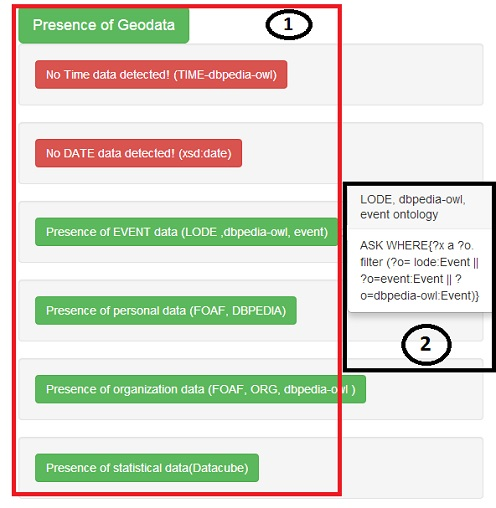
\includegraphics[width=0.4 \textwidth]{img/checkerCategory.png}
}
\subfigure[Overview of the report on categories detected. ]{
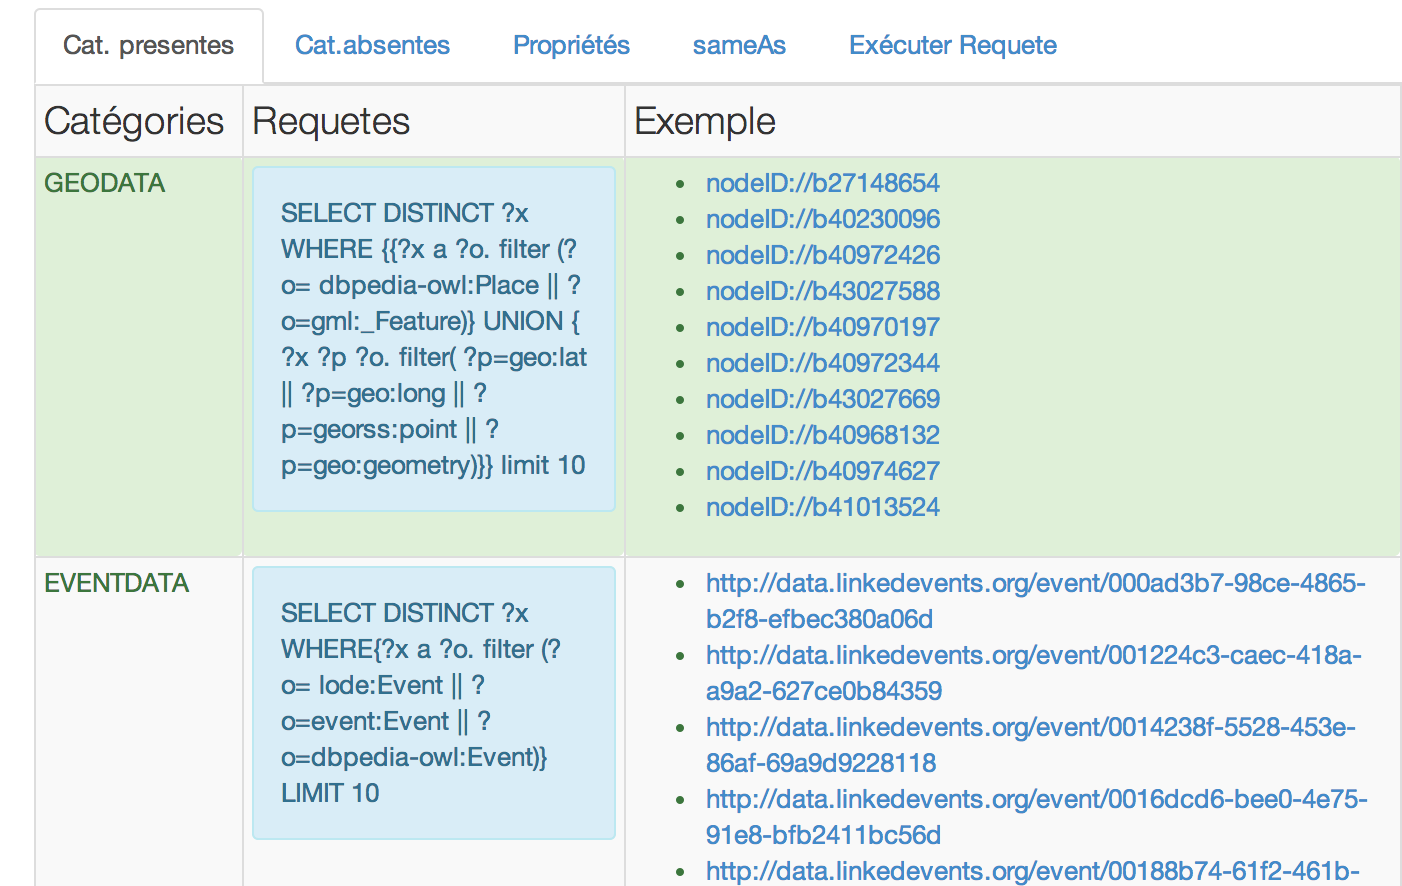
\includegraphics[width=0.4 \textwidth]{img/categories.png}
}
\subfigure[Two views generated by the LD wizard, for geodata and stats data]{
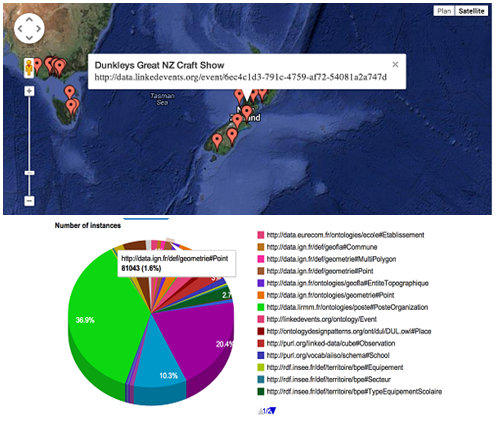
\includegraphics[ width=0.4 \textwidth]{img/samplevisu.png}
}


\caption{Categories detected and visualization generated by the Linked Data visualization wizard in the case of EventMedia endpoint service.}
\label{fig:visuSample}
\end{center}
\end{figure*}

\todo{Review Fig.6.2 b) }

\subsection{Conclusion}
\label{sec:conclusion-wizard}
In this Section we have presented  an approach for creating visualizations on top of Linked Data. We first defined seven categories of objects worth viewing in a dataset, and we propose to associate them with common Linked Data vocabularies. We then present a description of the main components of LDVizWiz: a Linked Data Visualization Wizard. We describe a lightweight implementation in javascript as a \textit{proof-of-concept} of our proposal, with the benefits to be usable on-line or being extensible. We advocate that such a tool can be easily integrated  in any workflow for publishing and linking data on the web, like Datalift\footnote{\url{http://www.datalift.org}} or the GeoKnow stack\footnote{\url{ http://generator.geoknow.eu/ }}. 

\section{A vocabulary for Describing VIsualization Applications} \label{sec:dvia}

We have implemented a vocabulary, DVIA\footnote{\url{http://bit.ly/Vb4L8k}} aims at describing any applications developed to consume datasets in 4-5 stars, using visual tools to showcase the benefits of Linked Data. It reuses four existing vocabularies: Dublin Core terms at \url{http://purl.org/dc/terms/}, dataset catalogue (DCAT) at \url{http://www.w3.org/ns/dcat#}, Dublin Core Metadata Initiative at \url{http://purl.org/dc/dcmitype} and the Organization vocabulary at \url{http://www.w3.org/ns/org#}.  It is composed of three main classes : 

\begin{itemize}
\item \textbf{Application}: This class represents the application or the mashup developed for demo-ing or consuming data in LD fashion. It is subclass of \textbf{dctype:Software}
\item \textbf{Platform}: The platform where to host or use the application, could be on the Web (Firefox, Chrome, IE, etc..) or mobile (android, iOS, mobile ) or even desktop
\item \textbf{VisualTool}: Represents the tool or library used to build the application. 
\end{itemize}

The diagram of the main classes and properties is depicted in Figure \ref{visuGraphModel}. The current version of the vocabulary in Turtle format can be found at \url{http://purl.org/ontology/dvia} .  Listing \ref{snapshot} is a snapshot of the description of the application which won the Semantic Web Challenge\footnote{\url{http://challenge.semanticweb.org/2012/winners.html}} in 2012, the \textit{EventMedia Live} application, described using DVIA vocabulary. It depicts apart from some metadata about the application (dct:title, dct:name, dct:issued, dct:creator and dct:license), the different visualization libraries integrated for building Eventedia Live (e.g.: Google API, Backbone, etc), as well as the operating systems where it is designed for, the different views/facets available in the application (map, charts, graphs, force-directed layout, ect) and the heteregeneous datasets used to implement it. 
\lstset{basicstyle=\scriptsize, backgroundcolor=\color{white}, frame=single, caption= {Snapshot in Turtle of the description of Event Media Live Application}, label=snapshot, captionpos=b}
\begin{lstlisting}

visuapp:eventMedia01
       a dvia:Application ; 
       dct:title "EventMedia Live"@en;   
       dvia:description "An application for reconciling Live events with media" ; 
       dvia:url <http://eventmedia.eurecom.fr> ; 
       dct:issued "2012-11-10"^^xsd:date ; 
       dvia:businessValue "not commercial" ;   
       dvia:keyword "events, media"^^xsd:string ; 
       dct:license <http://www.opendatacommons.org/licenses/pddl/1.0/> ; 
      dvia:platform [ a dvia:Platform ; 
			dct:title: "Desktop" ;
			dvia:preferredNavigator "Google Chrome" ; 
			dvia:alternativeNavigator "FireFox" ;
			dvia:system "Mac OS, Windows, Linux"^^string ] ; 
		
     dvia:usesTool [ a dvia:visualTool; dct:title "Google visualization Tool" ; 
	dct:description "Google visualization API" ; 
	dvia:accessUrl <https://developers.google.com/chart/interactive/docs/reference> ; 
	dvia:downloadUrl <http://www.google.com/uds/modules/gviz/gviz-api.js/> ] ;
    dvia:usesTool visuapp:visualTool02 ;
    dvia:consumes [ a dcat:Dataset; dct:title "BBC dump"] ; 
    dvia:consumes [ a dcat:Dataset; dct:title "last.fm scrapped dataset"] ;
    dvia:consumes [ a dcat:Dataset; dct:title "upcoming scrapped dataset"] ;
    dvia:consumes [ a dcat:Dataset; dct:title "eventful scrapped dataset"] ;
    dvia:consumes [ a dcat:Dataset; dct:title "Flickr scrapped dataset"] ;
    dvia:consumes [ a dcat:Dataset; dct:title "Music Brainz "] ;
    dvia:consumes [ a dcat:Dataset; dct:title "Foursquare Json file"] ;
    dvia:consumes [ a dcat:Dataset; dct:title "DBpedia"] ;
    dct:creator [foaf:mbox "khrouf@eurecom.fr"; foaf:name "Houda Khrouf"];
    dct:creator [foaf:mbox "vuk@eurecom.fr"; foaf:name "Vuk Milicik"];
    dct:creator [foaf:mbox "raphael.troncy@eurecom.fr"; foaf:name "Raphael Troncy"];
    dvia:view "map, chart, graph, force-directed layout" ; 
       .
	   ...
	
\end{lstlisting}

The full version of this sample description is available at \url{http://www.eurecom.fr/~atemezin/datalift/visumodel/eventMedia-sample.ttl}. The actual version of the DVIA intends to be small enough to cover the concepts that are needed to reuse partial or full parts of applications. 

\begin{figure}[!htbp]
\vspace{-2.5cm}
  \centering{
    %\leavevmode
      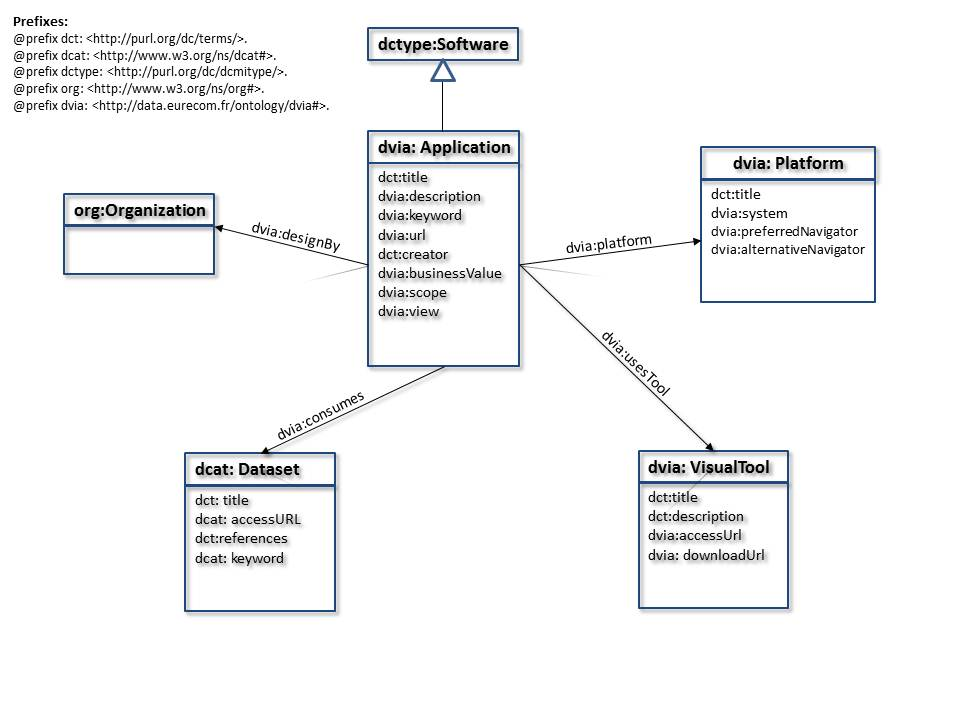
\includegraphics[ height=5in]{img/visuGraphModel.jpg}
  
    \caption{Conceptual Model of the DVIA vocabulary }
    \label{visuGraphModel}
  }
\end{figure}



\subsection*{Summary} \label{sec:conclusion}
% deploy the vocab and setting up a hub for mashups
% find patterns for applications
% develop a recommender for creating applications according to some criteria
\todo{Rewrite properly this section}
\textcolor{red}{We have presented in this paper an approach that could help reusing tools and libraries in the domain of applications built on top of datasets in Linked Open Data. We first presented our motivation as to demonstrate to the end users or decision makers, there is always a need to develop a showcase, hence sometimes looking for analogous or similar applications in the area to ease the process of creation the mashup. We proceeded by surveying some applications to extract relevant common facts worth reusable, from which we proposed a small vocabulary (DVIA)  to semantically describe visual applications. }

\textcolor{red}{We need to validate the DVIA by scrapping and reconciling data from all innovative applications websites and exposed them in RDF, starting with some of those we studied and others applications submitted at the Semantic Web Challenge the past three years. We strongly believe that having such a a hub  describing the tools, datasets, etc.  used to build  applications consuming 4-5 stars datasets will contribute to interoperable Applications leading to a Linked Open Visualizations (LOVIZ) on the LOD cloud.}


\section{Important Properties for an Entity}
\label{sec:propEntities}
In many knowledge bases, entities are described with numerous properties. However, not all properties have the same importance. Some properties are considered as keys for performing instance matching tasks while other properties are generally chosen for quickly providing a summary of the key facts attached to an entity. Our motivation is to provide a method enabling to select what properties should be used when depicting the summary of an entity, for example in a multimedia question answering system such as QakisMedia\footnote{\url{http://qakis.org/}} or in a second screen application providing more information about a particular TV program\footnote{\url{http://www.linkedtv.eu/demos/linkednews/}}. Our approach consists in: (i) reverse engineering the Google Knowledge Panel by extracting the properties that Google considers as sufficiently important to show (Section~\ref{sec:knowledge-graph}), and (ii) analyzing users' preferences by conducting a user survey and comparing the results (Section~\ref{sec:evaluation}). We finally show how we can explicitly represent this knowledge of preferred properties to attach to an entity using the Fresnel vocabulary~\cite{pietriga2006}. \\
\todo{TODO: ADD reference here?} \\
\todo{ADD figure of GKP search + result of crawling in JSON or implementation code}

\subsection{Reverse Engineering the Google KG Panel}
\label{sec:knowledge-graph}
Web scraping is a technique for extracting data from Web pages. We aim at capturing the properties depicted in the Google Knowledge Panel (GKP) that are injected in search result pages~\cite{Bergman2012}. We have developed a Node.js application that queries all DBpedia concepts that have at least one instance which is \texttt{owl:sameAs} with a Freebase resource in order to increase the probability that the search engine result page (SERP) for this resource will contain a GKP. We assume in our experiments that the properties displayed for an entity are type and context dependent (country, time, query) which can affect the results. Moreover, we filter out generic concepts by excluding those who are direct subclasses of \texttt{owl:Thing} since they will trigger ambiguous queries. We obtained a list of $352$ concepts\footnote{See also the SPARQL query at \url{http://goo.gl/EYuGm1}}.

\begin{algorithm}[h]\scriptsize
\caption{Google Knowledge Panel reverse engineering algorithm} \label{algoscrapping}
\begin{algorithmic}[1]
    \STATE INITIALIZE $equivalentClasses(DBpedia,Freebase) $ AS $vectorClasses$
    \STATE Upload $vectorClasses$ for querying processing
    \STATE Set $n$ AS number-of-instances-to-query
    \FOR {each $conceptType \in vectorClasses$}
	\STATE SELECT $n$ instances
	\STATE $listInstances \leftarrow$ SELECT-SPARQL($conceptType$, $n$)
		\FOR {each $instance \in listInstances$}
			\STATE CALL http://www.google.com/search?q=$instance$
			\IF {$knowledgePanel$ exists}
				\STATE SCRAP GOOGLE KNOWLEDGE PANEL
			\ELSE
				\STATE CALL http://www.google.com/search?q=$instance + conceptType$
 				\STATE SCRAP GOOGLE KNOWLEDGE PANEL
			\ENDIF
			\STATE $gkpProperties \leftarrow$ GetData(DOM, EXIST(GKP))
			
		\ENDFOR
	\STATE COMPUTE occurrences for each $prop \in gkpProperties$
    \ENDFOR
    \RETURN $gkpProperties$
\end{algorithmic}
\end{algorithm}
\normalsize
For each of these concepts, we retrieve $n$ instances (in our experiment, $n$ was equal to 100 random instances). For each of these instances, we issue a search query to Google containing the instance label. Google does not serve the GKP for all user agents and we had to mimic a browser behavior by setting the $User-Agent$ to a particular browser. We use CSS selectors to check the existence of and to extract data from a GKP. An example of a query selector is $.\_om$ (all elements with class name $\_om$) which returns the property DOM element(s) for the concept described in the GKP. From our experiments, we found out that we do not always get a GKP in a SERP. If this happens, we try to disambiguate the instance by issuing a new query with the concept type attached. However, if no GKP was found again, we capture that for manual inspection later on. Listing~\ref{algoscrapping} gives the high level algorithm for extracting the GKP. The full implementation can be found at \url{https://github.com/ahmadassaf/KBE}. We finally observe that this experiment is only valid for the English Google.com search results since GKP varies according to top level names.


\subsection{Evaluation}
\label{sec:evaluation}
We conducted a user survey in order to compare what users think should be the important properties to display for a particular entity and what the GKP shows.

\subsubsection{User survey.}
\label{sec:survey}
We set up a survey\footnote{The survey is at \url{http://eSurv.org?u=entityviz}} on February 25th, 2014 and for three weeks in order to collect the preferences of users in term of the properties they would like to be shown for a particular entity. We select only one representative entity for nine classes: \texttt{TennisPlayer}, \texttt{Museum}, \texttt{Politician}, \texttt{Company}, \texttt{Country}, \texttt{City}, \texttt{Film}, \texttt{SoccerClub} and \texttt{Book}. 152 participants have provided answers, 72\% from academia, 20\% coming from the industry and 8\% having not declared their affiliation. 94\% of the respondents have heard about the Semantic Web while 35\% were not familiar with specific visualization tools. The detailed results\footnote{\url{https://github.com/ahmadassaf/KBE/blob/master/results/agreement-gkp-users.xls}} show the ranking of the top properties for each entity. We only keep the properties having received at least 10\% votes for comparing with the properties depicted in a KGP. We observe that users do not seem to be interested in the \texttt{INSEE code} identifying a French city while they expect to see the \texttt{population} or the \texttt{points of interest} of this city.

\subsubsection{Comparison with the Knowledge Graphs.}
\label{sec:comparison}
The results of the Google Knowledge Panel (GKP) extraction\footnote{\url{https://github.com/ahmadassaf/KBE/blob/master/results/survey.json}} clearly show a long tail distribution of the properties depicted by Google, with a top N properties (N being 4, 5 or 6 depending on the entity) counting for 98\% of the properties shown for this type. We compare those properties with the ones revealed by the user study. Table~\ref{tab:agreement} shows the agreement between the users and the choices made by Google in the GKP for the 9 classes. The highest agreement concerns the type \texttt{Museum} (66.97\%) while the lowest one is for the \texttt{TennisPlayer} (20\%) concept. We think properties for museums or books are more stable than for types such as person/agent which vary significantly. We acknowledge the fact that more than one instance should be tested in order to draw meaningful conclusion regarding what are the important properties for a type.

\begin{table}[!htp]
\centering{\scriptsize
\begin{tabular}{lccccccccc}
\hline
 \textbf{Classes}	& TennisPlayer 	& Museum & Politician & Company & Country & City & Film & SoccerClub & Book	 \\ \hline
 \textbf{Agr.}& 20\%  & 66.97\% & 50\% & 40\% & 60\% & 60\% & 60\% & 50\% & 60\% \\ \hline
\end{tabular}
\caption{Agreement on properties between users and the Knowledge Graph Panel}
\label{tab:agreement}
}
\end{table}\normalsize

With this set of 9 concepts, we are covering $301,189$ DBpedia entities that have an existence in Freebase, and for each of them, we can now empirically define the most important properties when there is an agreement between one of the biggest knowledge base (Google) and users preferences.

\subsubsection{Modeling the preferred properties with Fresnel.}
\label{sec:fresnel}
Fresnel\footnote{\url{http://www.w3.org/2005/04/fresnel-info/}} is a presentation vocabulary for displaying RDF data. It specifies \textit{what} information contained in an RDF graph should be presented with the core concept \texttt{fresnel:Lens}. We use the Fresnel and PROV-O ontologies\footnote{\url{http://www.w3.org/TR/prov-o/}} to explicitly represent what properties should be depicted when displaying an entity. This dataset can now be re-used as a configuration for any consuming application.

\lstset{basicstyle=\scriptsize, backgroundcolor=\color{white}, frame=single, caption={Excerpt of a Fresnel lens in Turtle}, label=fresnel, captionpos=b}
\begin{lstlisting}
:tennisPlayerGKPDefaultLens rdf:type fresnel:Lens ;
  fresnel:purpose fresnel:defaultLens ;
  fresnel:classLensDomain dbpedia-owl:TennisPlayer ;
  fresnel:group :tennisPlayerGroup ;
  fresnel:showProperties (dbpedia-owl:abstract dbpedia-owl:birthDate
    dbpedia-owl:birthPlace dbpprop:height dbpprop:weight
    dbpprop:turnedpro dbpprop:siblings) ;
  prov:wasDerivedFrom
    <http://www.google.com/insidesearch/features/search/knowledge.html> .	
\end{lstlisting}
\normalsize

\section{Application consuming Event datasets: Confomaton}
\label{sec:confomaton}

In this Section, we aim at creating a rich environment to enable users to navigate events as well as their various representative media such as photos, slides and tweets. A typical usage is to gather data about a scientific conference and investigate the added value of collecting scientific related media. A non trivial task in such application is to connect structured data with extremely noisy content, especially in the case of a major conference.

 We consider a scientific conference, the International Semantic Web Conference (ISWC 2011), which took place in Bonn, Germany last November. Broadly speaking, considering all co-authors, people who have participated in the reviewing process, people who have physically attended the conference or tried to follow it on social networks, we estimate that it has attracted more than 1,500 participants. The conference organizers publish a lot of structured data regarding the conference including the list of accepted papers, their authors and institutions, the detailed program composed of sub-events with the exact timetable and the location (rooms) of the talks. This data is modeled using the SWC ontology\footnote{\url{http://data.semanticweb.org/ns/swc/ontology}}, which is designed to describe academic events, and uses classes and properties from other ontologies such as FOAF (for people) and SWRC (BibTeX elements for the papers). The main conference of type \texttt{swc:ConferenceEvent} is related to a set of sub-events, namely (\texttt{WorkshopEvent}, \texttt{TutorialEvent}, \texttt{SessionEvent}, \texttt{TalkEvent}) via the property \texttt{swc:isSuperEventOf}. Table~\ref{tab:dataset-stats} shows some statistics about the data provided by the Dog Food server regarding the ISWC 2011 conference. We first notice that the data is incomplete. The conference has hosted 16 workshops in total, but the 75 papers are only associated to 8 of them while the 8 others did not have any papers according to the corpus. Furthermore, we find 133 papers that are not connected to any of the events via the predicate \texttt{swc:hasRelatedDocument}. Finally, some useful information is also missing such as the keynote speakers and the \emph{Semantic Web Death Match} (panel) event. This lack of knowledge is also a motivation for our work: can we collect and analyse social network activities in order to complete the factual description of this event?

\begin{table}[htbp]
\footnotesize{
\begin{center}
\begin{tabular}{|r|r|r|r|r|r|}
\hline
\multicolumn{1}{|c}{\textbf{Main Event}} & \multicolumn{1}{|c}{\textbf{Sub-event}} & \multicolumn{1}{|c}{\textbf{Number of events}} & \multicolumn{1}{|c}{\textbf{Papers}} & \multicolumn{1}{|c|}{\textbf{Authors}}\\
\hline
& \texttt{Workshop Event} & 16 & 75 & 185\\
& \texttt{Tutorial Event} & 7 & 7 & 20\\
\texttt{Conference Event} & \texttt{Session Event} & 1 & 66 & 202\\
& \texttt{Talk Event} & 93 & 93 & 275\\
& - & - & 133 & 385\\
\hline
\texttt{Total (distinct)} & 4 & 117  & 292 & 735 \\
\hline
\end{tabular}
\vspace{1mm}
\caption{Metadata provided by the Dog Food Server for the ISWC 2011 conference.}
\label{tab:dataset-stats}
\end{center}}
\end{table}


We collected social network data in real time during the six days of the conference using the main tags advertised by the organizers (\texttt{\#iswc2011}, \texttt{\#cold2011}, \texttt{\#derive2011}, etc.). Table~\ref{tab:media-statistics} shows some statistics about the different media services used by the attendees along with the number of items from a number of distinct users. As expected, Twitter is by far the most used service: we have been able to collect 3,390 tweets from 519 different users. A significant proportion of tweets contains hyperlinks that we have further analysed. Hence, we extracted 384 different websites indexed by so-called URL shorteners (such as Bitly) found in 1,464 tweets (43\% of tweets). These links represent a rich source of media, as they pointed to various Web resources categories such as blogs, slides, photos, publications and projects. For example, 25\% of these links pointed to PDF documents that are generally one of the conference papers but could also be related papers relevant for the followers of the conference. We also analyse these links to extract the various media services used by Twitter.

\begin{table}[htbp]
\centering{
\begin{tabular}{|ll|r|r|}
\hline
\multicolumn{2}{|c}{\textbf{Media Service}} & \multicolumn{1}{|c}{\textbf{Items}} & \multicolumn{1}{|c|}{\textbf{Users}}\\
\hline
\multicolumn{2}{|l|}{Twitter} & 3390 tweets & 519\\
& \hspace{1em}pic.twitter & 12 photos &  6 \\
& \hspace{1em}yfrog  & 10 photos & 9 \\
\multicolumn{2}{|l|}{Twitpic} & 10 photos &  6 \\
\multicolumn{2}{|l|}{Flickr} & 47 photos & 6\\
\multicolumn{2}{|l|}{Google+} & 30 posts & 26\\
\multicolumn{2}{|l|}{Slideshare} & 25 slides & 20 \\
\hline
\end{tabular}
\vspace{1mm}
\caption{Media services used during ISWC 2011 conference}
\label{tab:media-statistics}
}
\end{table}

The name \emph{Confomaton} is a word play on the French term \emph{Photomaton} (English photo booth) and \emph{conference}. Just like a Photomaton illustrates the scene inside of the photo booth, the \emph{Confomaton} illustrates an event such as a conference enriched with social media. \emph{Confomaton} is a Semantic Web application that produces and consumes Linked Data and is composed of four main components (Figure~\ref{fig:architecture}): (i) an Event Collector that extracts events descriptions such as the ones available in the Semantic Web Dog Food corpus; (ii) a media collector that collects social media content and represents it in RDF using various vocabularies; (iii) a Reconciliation Module playing the role of associating social media with sub-events and external knowledge; (iv) a User Interface powered by an instance of the Linked Data API as a logical layer connecting all the data in the triple store with the front-end visualizations.

\begin{figure*}[t!h]
 \centering
 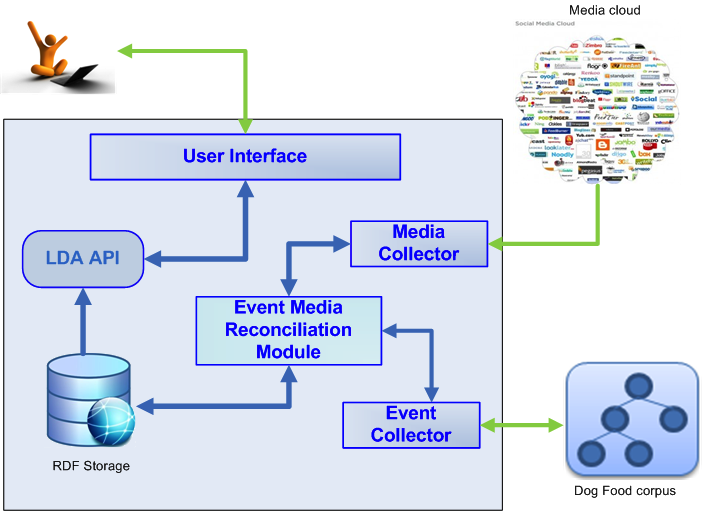
\includegraphics[scale=0.35]{img/architecture.png}
 \caption{\emph{Confomaton} general architecture.}
 \label{fig:architecture}
\end{figure*}


%%%  3.1 Media Collector  %%%
\subsection{Media Collector}                                                \label{sec:media-collector}
In the context of \emph{Confomaton}, we have developed so-called \emph{media collectors} with the purpose of searching various social networks and media platforms for event-related media items such as photos, videos, and slides. We currently support 4 social networks (Google+, MySpace, Facebook, and Twitter) and 7 media platforms (Instagram, YouTube, Flickr, MobyPicture, img.ly, yfrog and Twitpic). Our approach being agnostic of media providers, we offer a common alignment schema for all of them:
\begin{itemize}
  \item	\textbf{Media URI}, the deep link to the media item, e.g. \url{http://farm7.staticflickr.com/6059/6290784192_567346ba6a_o.jpg}
  \item \textbf{Type}, the type of the media item, e.g.  ``photo''
  \item \textbf{Story URI}, the URI of the micropost or story where the media item appeared, e.g. \url{http://www.flickr.com/photos/96628098@N00/6290784192/}
  \item \textbf{Message}, the concrete micropost or description text in raw format, e.g.  ``Laura. \texttt{\#iswc2011}, \texttt{\#semanticweb}, \texttt{\#bonn}, \texttt{\#germany}''
  \item \textbf{Clean}, the concrete cleaned micropost or description text with some characters (e.g. hash signs) removed, e.g. ``Laura. iswc2011, semanticweb, bonn, germany''
  \item \textbf{User}, the URI of the author of the micropost, e.g. \url{http://www.flickr.com/photos/96628098@N00/}
  \item \textbf{Published}, the timestamp of when the micropost was authored, or the media item was uploaded, e.g. \texttt{2011-10-27T12:24:41Z}
\end{itemize}

\begin{lstlisting}[caption={Sample output of the media collector showing Google+ and Flickr results using \#iswc2011 as query term},label={lst:media}]
{
  "GooglePlus": [
    {
	  "mediaurl": "http://software.ac.uk/sites/default/files/images/content/Bonn.jpg",
	  "storyurl": "https://plus.google.com/107504842282779733854/posts/6ucw1Udb5NT",
	  "message": {...}
    }],
    "Flickr": [
   {
      "mediaurl": "http://farm7.staticflickr.com/6226/6290782640_e8a1ffdcc2_o.jpg",
      "storyurl": "http://www.flickr.com/photos/96628098@N00/6290782640/",
      "message": {..}
    }]
 }
\end{lstlisting}

In order to retrieve data from media providers, we use the particular media provider's search Application Programming Interfaces (API) where they are available, and fall back to Web scraping the media provider's website if not. In some cases, we initially use the search API, but then have to fall back to Web scraping in order to get more details on the results, such as the \textbf{Media URI}, which is not exposed by all APIs. From all media providers, Twitter plays a special role, as it can serve as a host for other media providers. For example, it is very common for tweets to contain links to media items hosted on external media providers such as Twitpic. Other media providers treat media items as first class objects, i.e. have dedicated object keys in their API results for media items, which is not in all cases true for Twitter. We handle this by searching for a list of URIs of known media providers in combination with the actual search term. To illustrate this, when searching for media items for the search term ``ISWC 2012'' on Twitter, we would actually search for ``iswc 2012 AND (twitpic.com OR flic.kr)'' in the background, whereas on all other media providers, the search term ``iswc 2012'' is sufficient. The media collector can be tested at \url{http://webmasterapp.net/social/}.

\subsection{Data Modeling}
We have developed an Event Collector, which takes as input the Dog Food corpus described using the SWC ontology and converts all events into the LODE ontology\footnote{\url{http://linkedevents.org/ontology/}}, a minimal model that encapsulates the most useful properties for describing events. We use the Room ontology\footnote{\url{http://vocab.deri.ie/rooms}} for describing the various rooms contained in the conference centre. An explicit relationship between an event and its representative media (photo, slide, micropost, etc.) is realised through the \texttt{lode:illustrate} property. For describing those media, we re-use two popular vocabularies: the W3C Ontology for Media Resources\footnote{\url{http://www.w3.org/TR/mediaont-10/}} for photos and videos, and SIOC\footnote{\url{http://rdfs.org/sioc/spec/}} for tweets, status, posts and slides. The example below shows how a tweet is represented in \emph{Confomaton}.
{\footnotesize 	
\begin{verbatim}
<http://data.linkedevents.org/tweet/af557cef-5d5b-49c6-a4c3-bc9c41ce1555>
 a sioc:Post;
 dcterms:created "2011-10-23T13:34:03+00:00";
 sioc:content    "@smeh Good luck for your presentation at #ssn2011...";
 sioc:hasCreator <http://www.twitter.com/BadmotorF>;
 lode:illustrate <http://data.semanticweb.org/workshop/ssn/2011>;
 gc:hashtag      "#ssn2011";
 owl:sameAs      <http://twitter.com/BadmotorF/status/128071685235671040>.
\end{verbatim}
}

Figure~\ref{fig:natasha-example} depicts how all these vocabularies are used together. The ISWC 2011 conference is illustrated by a photo shared on Flickr, has for sub-event the EvoDyn 2011 workshop in which one of the tweets posted mentioned the recognised named entity Nathasha Noy who is also a general chair of the conference. All the data is available in the \emph{Confomaton} graph in a public SPARQL endpoint available at \url{http://semantics.eurecom.fr/sparql}.
\begin{figure*}[t!h]
 \centering
 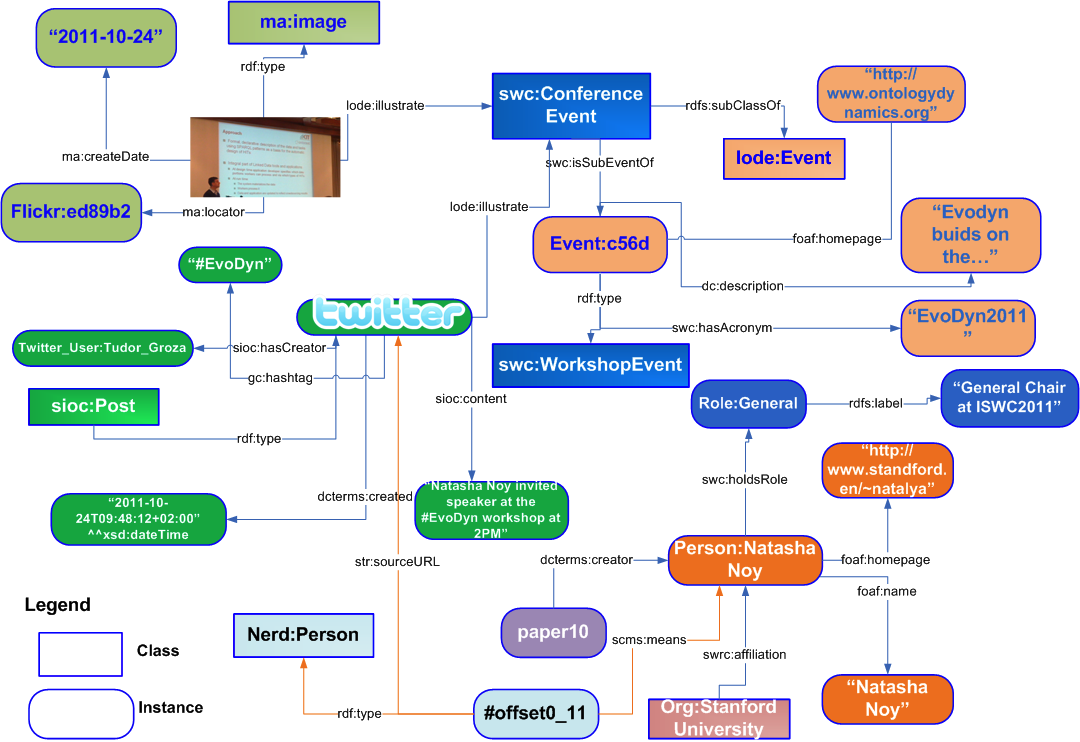
\includegraphics[scale=0.3]{img/natasha_example.png}
 \caption{Example of data modeled in \emph{Confomaton} re-using multiple vocabularies}
 \label{fig:natasha-example}
\end{figure*}



\subsection{Event Media Reconciliation Module}
The event media reconciliation module aims to align the incoming stream of social media with their appropriate events and to interlink some descriptions with general knowledge available in the LOD cloud\footnote{\url{http://lod-cloud.net/}} (e.g. people and institutions descriptions). Attaching social media to fine-grained events is a challenging problem. We tackle it by pre-processing the data with two successive filters in order to reduce the noise: one of them relies on keyword search applied to some fields such as title and tag, while the other one filters data based on temporal clues. The reconciliation is then ensured through a pre-configured mapping between a set of keywords and their associated events. This map enables us to associate media with the macro-events that people explicitly refer to in their posts or photos. For example, we connect all media items containing the tag \texttt{\#iswc2011} with the general ISWC 2011 conference. However, this method is absolutely not convenient to associate media items with sub-events. For instance, in the ISWC 2011 conference, there are 99 sub-events of type \texttt{TalkEvent}, which could be the presentation of a paper, a keynote speech or any other kind of talk. Social network users typically do not specify a particular tag for such events. We hence advocate the need for more advanced classifiers to associate media with sub-events. These classifiers can exploit a variety of parameters such as social network graphs and named entities extracted from media content. 

\subsection{Graphical User Interface}
The Graphical User Interface (GUI) of \emph{Confomaton} is built around four perspectives characterising an event: (i) \textit{``Where does the event take place?''}, (ii) \textit{``What is the event about?''}, (iii) \textit{``When does the event take place?''}, and finally (iv) \textit{``Who are the attendees of the event?''}. In addition, the user interface offers full text search for these four dimensions. The \emph{Confomaton} user interface is powered by the Linked Data API\footnote{\url{http://code.google.com/p/linked-data-api/wiki/Specification}}, which provides a configurable way to access RDF data using simple RESTful URLs that are translated into queries to our SPARQL endpoint. More precisely, we use the Elda\footnote{\url{http://code.google.com/p/elda}} implementation developed by Epimorphics. Elda comes with some pre-built samples and documentation, which allow to build specification to leverage the connection between the back-end (data in the triple store) and the front-end (visualizations for the user). The API layer helps to associate URIs with processing logic that extract data from the SPARQL endpoint using one or more SPARQL queries and then serialize the results using the format requested by the client. A URI is used to identify a single resource whose properties are to be retrieved or to identify a set of resources, either through structure of the URI, or through query parameters.

%\autoref{lst:config} shows an example of the configuration file of the \emph{Confomaton} API specifying the event, media and tweet viewers followed by the events and media properties access.
%\begin{lstlisting}[caption={Example configuration file of the \emph{Confomaton} API, specifying event properties access.},label={lst:config}]
%<#MyAPI> a api:API ;
%	rdfs:label "Confomaton API"@en ;
%	api:endpoint <#event>,<#media>,<#tweet>,<#agent>, <#venue>,<#user>,<#eventbyid>,<#mediabyid>,<#tweetbyid>,<#agentbyid>,<#venuebyid>,<#userbyid>;
%	api:sparqlEndpoint <http://semantics.eurecom.fr/sparql> ;
%# specification of the event viewer (all properties appear in the json file)
%spec:eventViewer a api:Viewer ;
%  api:property "title","description","space.lat","space.lon","time.datetime","inagent.label",...
%<#eventbyid> a api:ItemEndpoint;
%		api:uriTemplate "/event/{id}";
%		api:itemTemplate "http://data.linkedevents.org/event/{id}";
%		api:defaultViewer spec:eventViewer.		
%\end{lstlisting}

The system is available at \url{http://semantics.eurecom.fr/confomaton/iswc2011}. On the left side of the main view, the user can select the main conference event or one of the sub-events as provided by the Dog Food metadata corpus. In the centre, the default view is a map centred on where the event took place (e.g. Bonn, Germany) and the user is also encouraged to explore potential other types of events (concerts, exhibitions, sports, etc.) happening nearby, this data being provided by EventMedia~\cite{Troncy:ISEMANTICS10}. The \textit{What} tab is media-centred and allows to quickly see what illustrates a selected event (tweets, photos, slides). Zooming in an event triggers a popup window that contains the title and timetable of the event, the precise room location and a slideshow gallery of all the media items collected for this event. For the \textit{When} tab, a timeline is provided in order to filter events according to a day time period. Finally, the \textit{Who} tab aims at showing all the participants of the conference. This is intrinsically bound to a social component, aiming not only to present relevant information about participants (their affiliations, homepages, or roles at the conference), but also the relationships between participants themselves and with events.


\section{Application consuming Statistics datasets: PerfectSchool}
\label{sec:perfectSchool}

\subsection{Scope of the Application}
The \texttt{Perfect School} application is intended to provide useful information on schools in France using semantic technologies, with RDF-ized data enriched with other datasets in the wild. The application and the vocabulary have successfully passed the integrity checker\footnote{\url{http://www.w3.org/2011/gld/wiki/Data_Cube_Implementations}}  of an implementation for the candidate recommendation of Data Cube \url{http://www.w3.org/TR/vocab-data-cube/ } vocabulary at W3C.

\subsection{Legacy Datasets}
In order to build the application, we had to look at some relevant datasets in data.gouv.fr. The ones selected for building the application are the following:

\begin{itemize}
\item The file at \url{http://www.data.gouv.fr/DataSet/564055} in CSV format, containing a list of $67, 201$ schools (name, status, type), with geolocation position in Lambert 93, for the academic year 2011-2012. The file contains the following attributes (in French): 
	\begin{itemize}
		\item code of the school (e.g. 0010002X), 
		\item  official name of the school (e.g.: College Saint-Exupery), 
		\item principal name (e.g. COLLEGE), 
		\item patronymic name (e.g. Saint-Exupery), 
		\item status of the school (1 = open, 2 = to be closed and 3 = to be opened), 
		\item label of the type of school (e.g: 1= first degree, 3 = second degree).
	\end{itemize}
\item \url{http://www.data.gouv.fr/DataSet/572165}, in .CSV format giving results for professional schools, indicators), from one academic year (2011-2012). The file contains the following attributes:
	\begin{itemize}
		\item name of school, 
		\item  city code, 
		\item code of the school, 
		\item district where the school is located, 
		\item sector (PR= PRivate, PU= PUblic), 
		\item several observation measures with statistics on success rates, school versus academic/national rates, name of the academy it belongs to, as well as the department.
	\end{itemize}
   \item \url{http://www.data.gouv.fr/DataSet/572162} (.CSV) containing statistics for  $2296$ public high schools and indicators. It complements the statistics from INSEE.
\end{itemize}

\subsection{Ontology Modeling}
We have reused some external ontologies for more interoperability:
\begin{itemize}
\item \texttt{aiiso}\footnote{http://vocab.org/aiiso/schema} for the type of school and codes of school.
\item \texttt{geofla}\footnote{http://data.ign.fr/def/geofla\#} since the schools are considered as a topographic entities,
\item \texttt{geom}\footnote{http://data.ign.fr/def/geometrie\#} for representing the different geometries (points with latitude and longitude) in a given coordinate reference systems with \texttt{ignf} ontology at \url{http://data.ign.fr/def/ignf#} . 
\item \texttt{skos:Concept} for describing the 30 types of nature of schools. 
\item \texttt{qb:DimensionProperty}\footnote{http://www.w3.org/TR/vocab-data-cube/} and \texttt{qb:MeasureProperty} for modeling the dimensions and different indicators available for a given school. 
\end{itemize}
The resulting vocabulary is available at \url{http://purl.org/ontology/dvia/ecole}. 

We use the Datalift platform for transforming the different CSV files into RDF. The final data is available  at \url{http://eventmedia.eurecom.fr/sparql} with the named graph \texttt{http://data.eurecom.fr/school}.

\subsection{URI Policies}
We use the following patterns for the URIs of the vocabularies or the resources in our namespace.
\begin{itemize}
\item URI for vocabulary: \texttt{http://data.eurecom.fr/ontologies/\{SECTOR\}}. \\
e.g: \url{<http://data.eurecom.fr/ontologies/ecole>} for the ontology that we have developed.

\item URI for resources: \texttt{http://data.eurecom.fr/id/\{SECTOR\}/\{CLASS\}}. \\
e.g: \url{<http://data.eurecom.fr/id/school/>} for the schools URIs, \\
\url{<http://data.eurecom.fr/id/school/slice/>} for \texttt{qb:Slice}s.

\item URI for taxonomies: we use \texttt{SKOS} for modeling concepts and codes as the following: \\
\texttt{http://data.eurecom.fr/codes/\{SECTOR\}/\{CONCEPT-TYPE\}/\{CODE\}}. 
e.g.: \url{<http://data.eurecom.fr/codes/ecole/natureUAI>} for the collection of natures of the schools ; \\
        \url{<http://data.eurecom.fr/codes/ecole/natureUAI/101>} for a particular concept with code \textit{101} and label '''\'{E}cole maternelle".

\end{itemize}

Besides the aforementioned policy, each school in the user interface can be reached on the UI by using directly the following URI: 
 \url{http://semantics.eurecom.fr/datalift/PerfectSchool/#school/{SCHOOL-CODE/}}, with \{SCHOOL-CODE/\} in lowercase. 
 
\paragraph{\textit{Example:}}
\textit{The school ``Albert Camus'' in the city ''Le Mans'' with the code school $0720800D$ can we viewed in the application directly at} \url{http://semantics.eurecom.fr/datalift/PerfectSchool/#school/0720800d/}

\subsection{Sample School Data in RDF }

\lstset{basicstyle=\scriptsize, backgroundcolor=\color{white}, frame=single, caption= {Snapshot in Turtle for the school ID=0750676C, also at \url{http://semantics.eurecom.fr/datalift/PerfectSchool/\#school/0750676c/}}, label=snapshot, captionpos=b}
\begin{lstlisting}

school:0750676c 	a	aiiso:School,  geofla:EntiteTopographique .
school:0750676c 	a	ecole:Etablissement .
school:0750676c	rdfs:label	"LYCEE DORIAN (PROFESSIONNEL)"@fr ;
school:0750676c	dcterms:title	"Lycee polyvalent et lycee des metiers de la .."@fr ;
	aiiso:code	"0750676C" ;
	ecole:denominationPrincipale "LPO LYCEE DES METIERS"@fr ;
	ecole:patronyme	"DORIAN"@fr ;
	ecole:ville	"PARIS 11"@fr ;
	ecole:codeCommune	"75111" ;
	ecole:secteur	"PU" ;
	ecole:academie	"PARIS"@fr ;
	ecole:departement	"PARIS"@fr ;
	ecole:cycle	"3"^^xsd:int ;
	ecole:etat	"1"^^xsd:int ;
	ecole:nature	bpenat:306 .

slice:0750676c	ecole:etablissement	school:0750676c .
school:0750676c	geom:geometrie	_:vb42480647 , _:vb42531960 .		 

_:vb42480647 a geom:Point;
	geom:systCoord ignfr:wgs84g;
	geom:coordX "48.85429801"^^xsd:double;
	geom:coordY "2.39231163"^^xsd:double . 

_:vb42531960 a  geom:Point;
	geom:systCoord ignfr:ntflamb2e ;
	geom:coordX "655410.1"^^xsd:double;
	geom:coordY "6861755.9"^^xsd:double .
     
	
\end{lstlisting}

\subsection{Interconnection}
For the interconnection process, we didn't use the current module. Instead of that we have used the Silk \cite{jentzsch2010silk} platform as it is re-packaged in the workflow of Datalift. We believe the scripts used for this task can be easily reused within the Datalift platform. Two datasets where used for finding \texttt{owl:sameAs} links:
\begin{enumerate}
\item DBpedia French chapter\footnote{\url{http://fr.dbpedia.org/sparql}}, as the scope of the application was limited to France. We have found only 7 match links with our schools datasets.
\item LinkedGeoData\footnote{\url{http://linkedgeodata.org/sparql}}, as the underlying data used comes from the community project Open Street Map (OSM). Here, we got  a total of $601$ matching links in the category of \texttt{lgdo:BuildingSchool}\footnote{\url{http://linkedgeodata.org/ontology/BuildingSchool}}. 
\end{enumerate}

\subsection{User Interface}
The target device for the application is Mobile phone, using principally two frameworks: Jquery mobile\footnote{http://jquerymobile.com/} and  backbone javascript\footnote{\url{http://backbonejs.org/}}. 
The application provides geolocation, search by city/district, graph charts for stats, table views of relevant results aggregated or group by some other aspects. 
\texttt{Perfect School Application} provides 3 main views:
\begin{enumerate}
\item \textbf{Search form:} The interface retrieves the location automatically ( \'{a} la Google Maps API fashion) , and offers box choices based on the School type: First degree / second degree. When choosing first degree, the user can further select one of (primary school, elementary school or other). For the second degree, apart from looking for one of College, high school or other, the user can look for public or private schools. The search button launches the query behind the scene for retrieving the collection of data matching the user's criteria. 

\item \textbf{Results of searching}: The search action returns a collection of schools plotted in a map. A cursor on the left side helps users zoom to get more details about schools retrieved in a given region, or street. When selecting a given school, the name is displayed and with the possibility to see the route from the barycenter of the result on the map.
\item \textbf{Description of the school:} It is divided in 3 different tabs: (a) General information (name, cycle, principal denomination, nature and patronym used) ; (b) Stats with all the different statistics in form of charts, graphs comparing the school with the others ; and (c) DBpedia-FR\footnote{\url{http://fr.dbpedia.org}} information if available, obtained with the \texttt{owl:sameAs} links for enriching the original dataset with  information such as founder, date of creation, web site, population, head of school etc.

\end{enumerate}

The Figure ~\ref{fig:searchingSchool} shows the three different views on a running example.


\begin{figure*}[!htbp]
\begin{center}
\subfigure[Search options]{
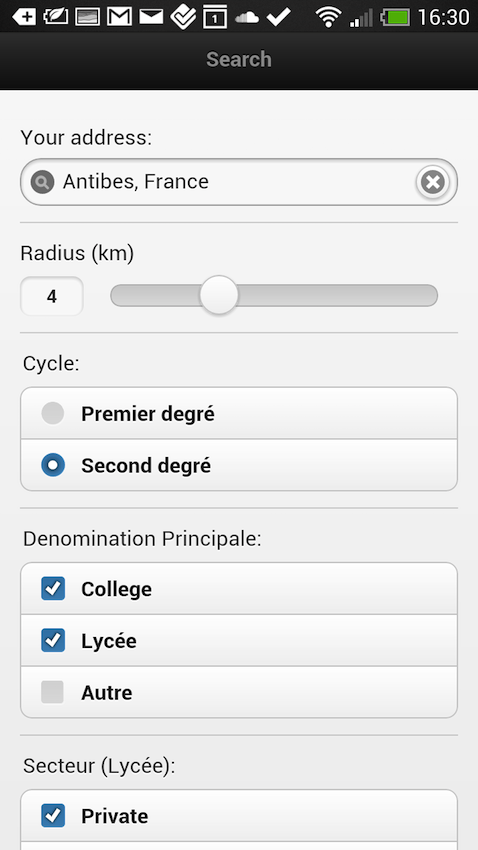
\includegraphics[height=62mm,width=42mm]{img/searching.png}
}
\subfigure[Results displaying on a map]{
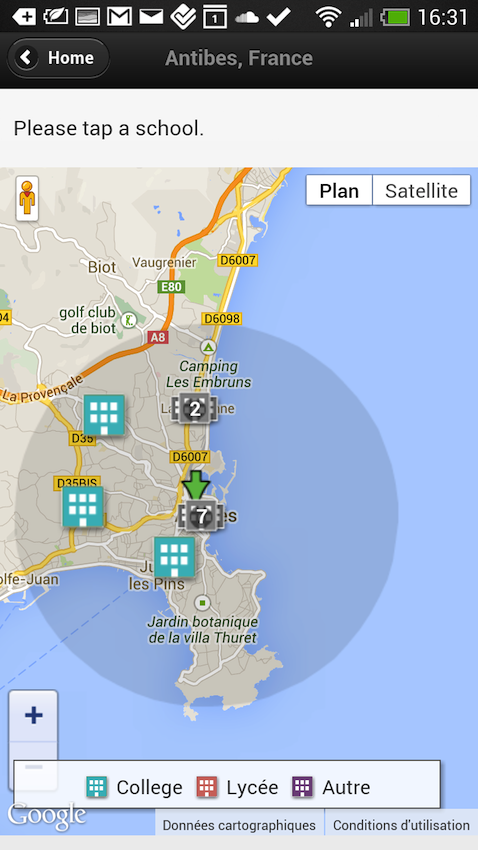
\includegraphics[height=62mm,width=42mm]{img/result.png}
}
\subfigure[Route to the selected school]{
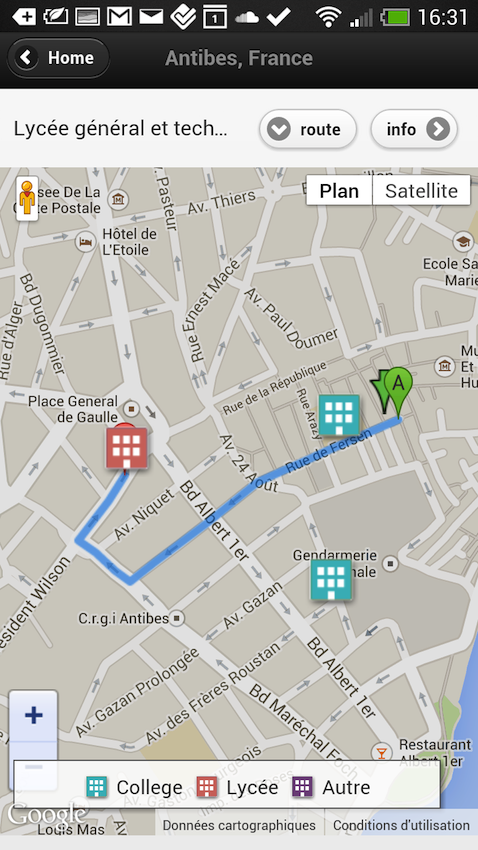
\includegraphics[height=62mm,width=42mm]{img/routeresult.png}
}
\subfigure[Details information with 3 tabs: General, statistics and DBpedia]{
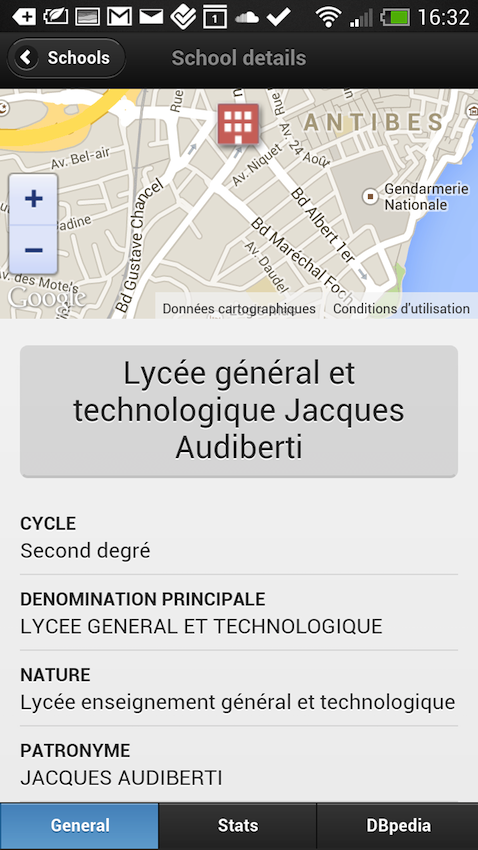
\includegraphics[height=62mm,width=42mm]{img/tab-result.png}
}
\caption{Steps for searching high schools in Antibes in a radius of 4000m, France}
\label{fig:searchingSchool}
\end{center}
\end{figure*}



\section{Improving the discovery of applications contests in Open Data Events}
\label{sec:contests}

\todo{add Alexis work + add appendix of content scrapping and JS apps installation }

\subsection{Background}
\label{sec:backcontest}

\subsection{Modeling events and applications in RDF}
\label{sec:modeleventsapps}

\subsection{Universal JavaScript plugin for RDF population}
\label{sec:plugin}

\subsection{Creating the Knowledge-base for past events}